\section{Kapitel 1}


\subsection{Management Summary}

TODO

\subsection{Motivation}

\begin{quote}
"`Prozessorientierung ist seit Beginn der 90er Jahre als eine unverzichtbare 
Maxime der Unternehmensgestaltung akzeptiert. In den letzten Jahren 
haben viele Unternehmen Maßnahmen
 zur verstärkten Ausrichtung an ihren Geschäftsprozessen initiiert."' 
\footcite[S.182]{prozessmanagement:leitfaden}
\end{quote}


Aussagen wie diese, zeigen dass die Prozessorientierte
Geschäftsprozessmodelierung mittlerweile fest in allen Unternehmen angekommen ist.
Umso wichtiger ist es also, die Unterschiede und Feinheiten verschiedener Tools,
Prozesse und Anwendungsszenarien zu kennen.

\subsection{Ziel der Arbeit}

Die vorliegende Arbeit soll dem Leser einen vollständigen Überblick über die
Kernbereiche der Prozessmodelierung geben. Hierzu wird zunächst auf die
Entstehung und Notwendigkeit der Prozessorientierung eingegangen. Anschließend
sollen Vertiefungen der Methodik ein genaueres Verständniss erzeugen woraufhin
einige bekannte Software-Tools präsentiert werden.

\clearpage
\section{Geschäftsprozesse}

\subsection{Prozess}


Ein „Prozess“, vom lateinischen „processus“ („Fortgang, Fortschreiten“) ist von
der Wiederholung bereits existierender Vorgänge geprägt.

Es handelt sich dabei also um eine sich äufig wiederholte, eher sequentielle
Verkettung von Aktivitäten, wobei die Ausgangslage sowie das
angestrebte Ergebnis definiert und die erforderlichen Maßnahmen
kategorisiert bzw. spezifiziert sind. Dabei besetehen stets nur
unbedeutende Unsicherheiten in der Zielerreichung zum Beispiel "`Beschaffung
eines Zulieferteils"'.

\subsection{Definition und Management von Geschäftsprozessen}


Ein Geschäftsprozess besteht aus der wiederkehrenden Abfolge von logischen,
zeitlich zusammengehörigen und inhaltlich abgeschlossenen Aktivitäten, dessen 
Durchführung als Ziel die Wünsche der Kunden, die ein Unternehmen besitzt, zu befriedigen trägt.
Eine höhere Kundenzufriedenheit bedeutet ebenfalls eine höhere Wertschöpfung. 
Mit einem bestimmten Input und bestimmtem Ressourceneinsatz, 
entsteht ein Output, der an einen Empfänger geht. 
Dieser Empfänger kann ein Kunde, ein Lieferant oder eine innerbetriebliche Stelle sein. 
Handelt es sich tatsächlich um einen innerbetrieblichen Prozess, 
so kann davon ausgegangen werden, dass dieser organisatorisch dauerhaft geregelt wird.
\footcite[Vgl.][ ]{prozess:db}\\



Zusätzlich wird unterschieden zwischen Leistungs-, Unterstützungs- und
Führungsprozessen den sogenannten Prozessarten. Prozesse werden analysiert, 
woraus eine Bewertung ihrer Funktionalität und Effektivität entsteht. 
Ziel der Prozessanalyse ist vor allem die Schaffung einer Transparenz als 
Voraussetzung für eine bestmögliche Prozesssteuerung, dem „Geschäftsprozessmanagement“. 
Eine einfache Wortanalyse ergibt, dass sich das Geschäftsprozessmanagement 
mit der Verwaltung von Geschäftsprozessen beschäftigt.
\footcite[S.13]{lehmann}\\

Dazu zählen insbesondere folgende Aspekte:
Identifikation, Planung, Dokumentation,  Gewichtung, Verbesserung,
Steuerung, Kontrolle und Organisation von Geschäftsprozessen.
Zusammengefasst ist das Hauptziel und damit allgemeine Anforderung in Unternehmen, 
alle Prozessaktivitäten und Prozesse möglichst effizient auszuführen. 
Die Herausforderung für Unternehmen besteht darin, dass diese 
möglichst unterbrechungs- und fehlerfrei ablaufen.\\

Wenn die Prozesse und Unterprozesse einmal identifiziert worden sind, 
erfolgt die Beachtung der oben genannten Aspekte in Form einer Modellierung. 
Ein Prozessmodell dient dazu die kombinierte, überschneidungsfreie 
und lückenlose Struktur zusammenhängender Prozesse in einem Unternehmen darzustellen. 
Hierzu gibt es verschiedene Möglichkeiten. 
Im einfachsten Fall werden textuelle oder tabellarische Beschreibungen verwendet. 
Häufig werden Präsentations- oder Grafikprogramme genutzt, um einfache Ablaufdiagramme 
zu erstellen. Sie bestehen meist aus Kästchen und Pfeilen, wobei keiner 
bestimmten Methodik gefolgt wird.\\
Zur genauen Darstellung komplexerer Prozesse mit allen relevanten Aspekten, 
wie Verzweigungsregeln, 
Ereignissen, ausführenden Organisationseinheiten, Datenflüssen usw., 
genügt eine grobe Modellierung nicht. Hierfür werden geeignete Notationen benötigt. 
Mit welchen Symbolen die verschiedenen Elemente von Prozessen dargestellt werden, 
was sie genau bedeuten und wie sie miteinander kombiniert werden können, 
wird durch die Notation festgelegt. (Prozessmodellierung)
Welche Merkmale in Prozessmodellen abgebildet werden, hängt vom 
Modellierungszweck und der verwendeten Modellierungssprache ab. 
Die Regeln zur Modellierung von Geschäftsprozessen werden in folgenden Kapiteln deutlich.

\clearpage
\section{Prozessmodellierung und Notationen}

Im Zuge der Modellierung hat man es mit Zeichen unterschiedlichster Art zu tun.
Prozessmodelle können in Form von Texten, Tabellen oder Grafiken dargestellt werden. 
Üblicherweise wird eine Modellierungssprache verwendet, 
die eine Notation zur Abbildung von Geschäftsprozessen zur Verfügung stellt. 
In dieser Arbeit wird insbesondere mit der Notation BPMN gearbeitet.

\subsection{Ereignisgesteuerte Prozesskette}

EPK ist als Abkürzung einer ereignisgesteuerten Prozesskette zu verstehen und
ist für die detaillierte Modellierung und Veranschaulichung
von Geschäftsprozessen und Prozesselementen gut
geeignet.\footcite[Vgl.][]{lehmann}
 

Diese Notationsform ist 1992 unter der Leitung von
Scheer\footcite[Vgl.][]{scheer} entwickelt worden, somit wird die Bezeichnung
Sheer-Notation oft verwendet.
EPKs sind das Hauptdarstellungsmittel in Architecture of Integrated 
Information Systems (ARIS), darunter Ereignisse, 
Funktionen und Verknüpfungsoperatoren. Es gibt ebenfalls eine erweiterte EPK, 
die weitere Merkmale, wie bspw. Organisationseinheiten, Rollen von Mitarbeitern, 
sowie Datenbestände bzw. Informationssysteme, bietet. 
Da die Entwicklung und Pflege sehr umfangreich werden können ist die 
Nutzung von Softwarewerkzeugen notwendig. 
ARIS unterstützt Unternehmen bei der Modellierung, Analyse und Optimierung von Prozessen.
Das Grundproblem, nämlich der steigende Wettbewerbsdruck bezüglich der Zeit, 
Kosten und Qualität verlangt effiziente und effektive Organisationsformen. 
Unter einer Prozessorganisation ist nun eine Organisationsform zu verstehen, 
bei der die Strukturierung von organisatorischen Einheiten, 
insbesondere  Prozessteams bzw. Funktionsbereiche, 
den Kern- und Unterstützungsprozessen folgt.

\subsection{Business Process Model and Notation}

\begin{quote}
"`BPMN ist ein Standard und soll die Brücke zwischen Business und IT schlagen."'
\footcite[Vgl.][]{praxishandbuch:bpmn2}
\end{quote}

Business Process Model and Notation (BPMN) ist eine grafische 
Spezifikationssprache in der Wirtschaftsinformatik und im Prozessmanagement.
\footcite[Vgl.][]{allweyer}

Es ist der Standard für graphische und XML-basierte
Geschäftsprozessmodellierung. 
Mit seinen Symbolen und Elementen ist eine einheitliche, standardisierte Sprache,
Darstellung und Analyse der Prozesse möglich. 
Im Gegensatz zu EPK könnte man BPMN als eine „junge Modellierungsnotation“ bezeichnen. 
Sie wurde von dem IBM-Mitarbeiter Stephen A. White im Jahr 2002 entworfen, 
daraufhin von der Business Process Management (BPM) 
Initiative veröffentlicht und im Jahr 2005 an die Object Management Group (OMG) 
zu einem Modellierungsstandard erklärt.

Um BPMN verstehen zu können, muss zunächst das Verständnis für BPM geschaffen
werden. BPM ist ein systematischer Ansatz, der
dazu dient sowohl automatisierte als auch nicht-automatisierte 
Prozesse zu erfassen, zu gestalten und auszuführen. 
Stattdessen wird häufig auch der Begriff Geschäftsprozessmanagement dafür
verwendet.\footcite[S.1]{praxishandbuch:bpmn2}
 
Mit Hilfe von BPM können Prozesse auf die Unternehmensstrategie abgestimmt werden, 
sodass sich die Gesamtunternehmensleistung verbessert, sobald Prozesse innerhalb 
einzelner Organisationseinheiten, unternehmensweit oder sogar unternehmensübergreifend 
optimiert werden.

Zunehmend werden für die Ausführung von Prozessen Business Process Management-
Systeme (BPMS) eingesetzt. Ein BPMS enthält eine Process Engine, 
die die Abläufe direkt anhand geeigneter Prozessmodelle oder 
formaler Prozessbeschreibungen steuert. 
Hierfür müssen die Modelle besonders strikten Anforderungen genügen, 
da sie nicht von Menschen in ein Computerprogramm umgesetzt, 
sondern direkt von einer Maschine abgearbeitet werden.

In Abhängigkeit von der Situation, den Ansprüchen und Zielen der einzelnen
Unternehmen ergeben sich vielfältige Nutzenpotenziale 
durch die Anwendung von BPMN. Es wird die verständliche Definition 
und Dokumentation von Prozessen für die tägliche Anwendung und zur 
Orientierung von Managern und Mitarbeitern geschaffen. 
Zudem werden das Modell und die Notation standardisiert und stellen eine 
gleiche Interpretation der gegebenen Prozessdefinition 
von allen Prozessbeteiligten sicher. Verbesserung der Zusammenarbeit 
zwischen Fachabteilung und IT-Dienstleister durch eine 
anschauliche graphische Prozessmodellierung einerseits und eine präzise 
Prozessdarstellung entsprechend einer Prozessgrammatik andererseits.1
\footcite[S.1]{allweyer}

Die Effizienz wird dadurch gesteigert, dass Mehrfach-Arbeit vermieden wird und
die Zuständigkeiten und Abläufe klar definiert sind. 
Entscheidend für eine erfolgreiche Umsetzung ist immer der konkrete Nutzen, 
der sich direkt für Unternehmen oder Institutionen und deren Mitarbeiter ableitet.


\subsection{Sprachelemente und Konventionen}

\subsubsection{EPK}

EPK beschreibt die Ablauforganisation eines Unternehmens, wobei die logische
Abfolge sowie das Zusammenwirken von Prozesselementen, Daten,
Informationssystemen, Organisation sowie Erzeugnissen dargestellt werden.

\begin{figure}[H]
\begin{minipage}{\linewidth}
\begin{center}
\fbox{
\centering
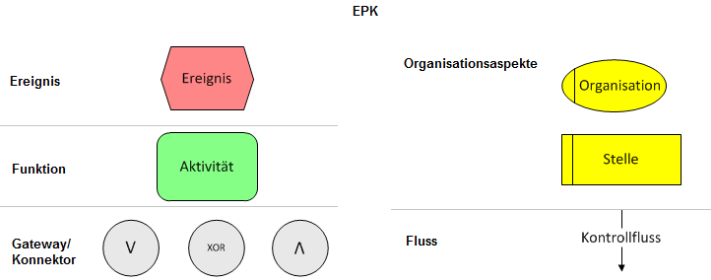
\includegraphics[width=13cm]{images/epk.png}
\caption{
EPK-Elemente
\newline
}
}
\end{center}
\end{minipage}
\end{figure}


Ein Ereignis repräsentiert sowohl einen Ausgangs- als auch einen Endpunkt.
Dieses bestimmt auch welche Zustände bzw. welche Bedingungen einen Prozess 
auslösen und welche Zustände die Beendigung eines Prozesses definieren.

\subsubsection{BPMN}

Aus der folgenden Grafik kann man entnehmen, dass BPMN auf sehr ähnliche
Notationselemente zurückgreift, jedoch fordert es nicht nur 
fachliche Prozessdokumentation, sondern auch informationstechnologische 
Konventionen zu berücksichtigen.

\begin{figure}[H]
\begin{minipage}{\linewidth}
\begin{center}
\fbox{
\centering
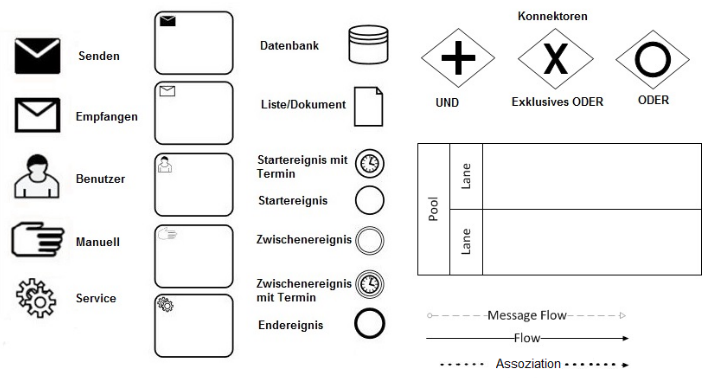
\includegraphics[width=13cm]{images/bpmn.png}
\caption{
BPMN-Elemente
\newline
}
}
\end{center}
\end{minipage}
\end{figure}

Die BPMN-Elemente werden insgesamt in fünf Kategorien eingeteilt: Flussobjekte
(Aktivitäten, Senden, Empfangen etc.), Verbindende Objekte 
(Message Flow, Flow, Assoziation etc.), Daten (Datenobjekt, Liste, Dokument etc.), 
Swimlanes (Pool, Lanes) und Artefakte (Gruppierungen, Anmerkungen etc.).

Ein Prozess wird häufig für eine (juristisch) selbstständige  Geschäftseinheit
(Business Unit) oder Organisation modelliert. Eine solche Geschäftseinheit 
kann Teilnehmer (participant) an einer Zusammenarbeit zwischen zwei, 
oder mehreren Geschäftspartnern sein. Der "`Pool"'  dient als grafische 
Darstellung einer selbstständigen Business Unit bzw. eines Teilnehmers 
an einer Zusammenarbeit. Die Lanes darunter können als sogenannte "`Schwimmbahnen"'
Swimlanes gesehen werden. Diese können untergeordnete Partnerrollen 
(z.B. Vertrieb, Projektleitung, Beschaffung, Bereich) oder Komponenten 
eines Systems sein und sie zeigen für welche Aktivitäten sie verantwortlich sind. 
Der Pool ist den Lanes übergeordnet und enthält die Lanes.\\

Ein Prozess startet und endet in der Regel mit einem Ereignis (Startereignis
bzw. Endereignis). BPMN schreibt nicht zwingend vor, wie und ob Start- 
und Endereignisse zu modellieren sind, es hilft jedoch zum besseren Verständnis. 
Ereignisse werden durch einen Kreis dargestellt, je nach Art- eine schmale 
unterbrochene, oder eine dicke durchgezogene Kreislinie- gekennzeichnet. 
Die Aktivitäten können als Kern eines Prozesses verstanden werden. 
Sie stellen ein Rechteck mit abgerundeten Ecken dar und werden am 
sinnvollsten mit einer „Objekt+Verb“-Verbindung (z.B Verfügbarkeit prüfen) 
beschriftet. Gateways dagegen sind als Kontrolle, Steuerung von Prozessen 
und als Verbindung zwischen Aktivitäten zu verstehen. Für diese wird die 
Raute als Zeichen verwendet, welches je nachdem, welche Entscheidungsmöglichkeit 
es gibt, mit einem X, einem XOR oder einem OR beschriftet wird.\\

In welcher Reihenfolge die vorgenannten Elemente durchlaufen werden bestimmen
die "`Sequenzflüsse"' (sequence flow). Es handelt sich hierbei um einen 
durchgängigen Verbindungspfeil mit "`ausgefüllter"' Spitze, welches jedoch nur 
innerhalb eines Pools, auch Lane-übergreifend, verwendet werden kann. 
Der Austausch zwischen den Pools dagegen geschieht durch "`Nachrichtenflüsse"' (message flows),
 welche durch einen "`gestrichelten"' Verbindungspfeil mit leerer Spitze gekennzeichnet 
 sind. Hierbei sind noch einige Regeln zu beachten: Nachrichtenflüsse können nur mit 
 sendenden oder empfangenden Nachrichten-Ereignissen verbunden werden. 
 Nachrichtenflüsse dürfen zudem nicht in ein Nachrichten-Ereignis hinein- und 
 gleichzeitig wieder herausführen, da jedes Nachrichten-Ereignis entweder sendend 
 oder empfangend ist und nicht gleichzeitig beides.\\


In der Praxis kommen häufig komplexe Prozessmodelle vor. 
Um die Brücke zwischen Business und IT zu schlagen, 
können mit Hilfe von BPMN Geschäftsprozesse verständlicher und ausführbar 
beschrieben und entworfen werden.\\




\clearpage
\section{Software für BPMN-Modelierung}

Im Laufe der Zeit haben sich immer mehr Anbieter am Markt etabliert, die
Lösungen zur Modellierung mit BPMN anbieten. Allein in der Wikipedia-List
befindet sich eine Auflistung von 25 Unternehmen.\footcite{wikitools}
Im folgenden werden einige Produkte beschrieben und miteinander
verglichen.

\subsection{ARIS Express}

ARIS Express wird von der Darmstädter Software AG seit 2009 entwickelt und
vertrieben. Die Software wird als "`freeware"' vertrieben wodurch die
grundsätzliche Nutzung kostenfrei ist.

\begin{figure}[H]
\begin{minipage}{\linewidth}
\begin{center}
\fbox{
\centering
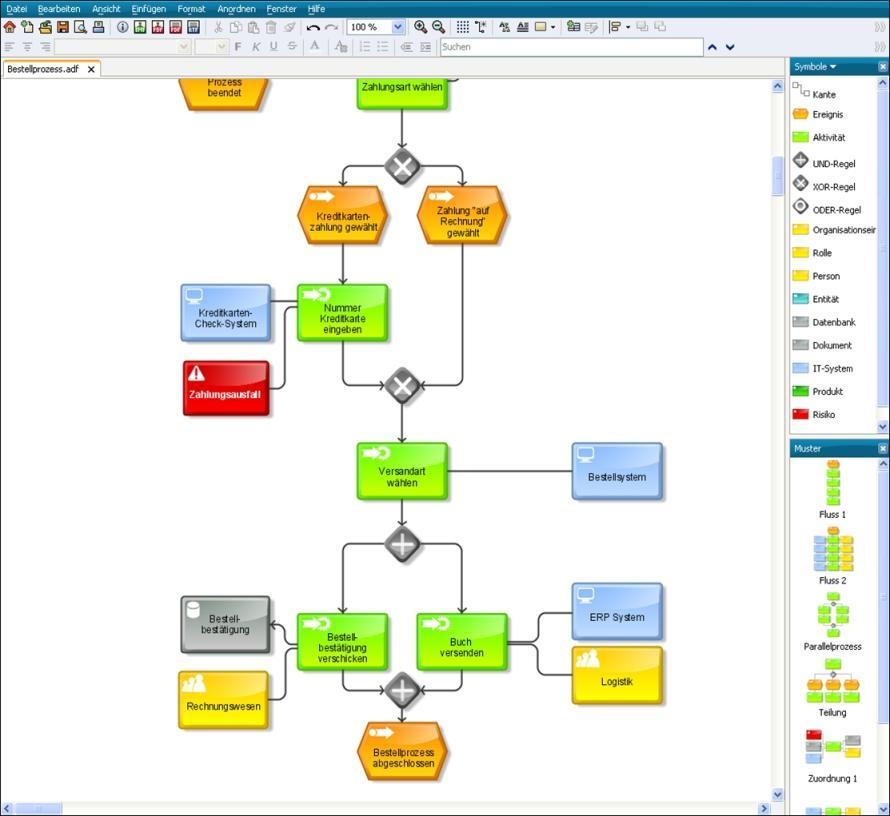
\includegraphics[width=13cm]{images/aris.jpg}
\caption{
Screenshot von ARIS Express
\newline
Quelle: {\protect\url{
https://www.computerwoche.de/i/detail/artikel/1928049/1/940760/d2e73-media/
}}\newline
Aufruf: 13.12.2017
}
}
\end{center}
\end{minipage}
\end{figure}


ARIS läuft dabei als Java-Applikation
auf dem Rechner des Nutzers wodurch es möglich ist, das Tool sowohl auf Windows-
als auch auf Linux- und Mac-Betriebssystemen zu nutzen.
Hierbei ist neben BPMN 2.0 auch die Nutzung von eventgetriebenen
Prozessketten (EPC), Organisationsdiagrammen, 
Prozesslandschaften und Whiteboards möglich.\\

Beachtenswert ist vor allem das intuitive Bedienungskonzept.
Auch ohne Einführung und Vorkentnisse ist es dem Nutzer bereits möglich einfache
Prozessketten abzubilden.


\subsection{Bonita BPM}

Bonita ist eine Open-Source-Software welche seit 2001 entwickelt wird. Der
Quellcode ist dabei unter github einseh- und änderbar.\footcite{bonitasource}

\begin{figure}[H]
\begin{minipage}{\linewidth}
\begin{center}
\fbox{
\centering
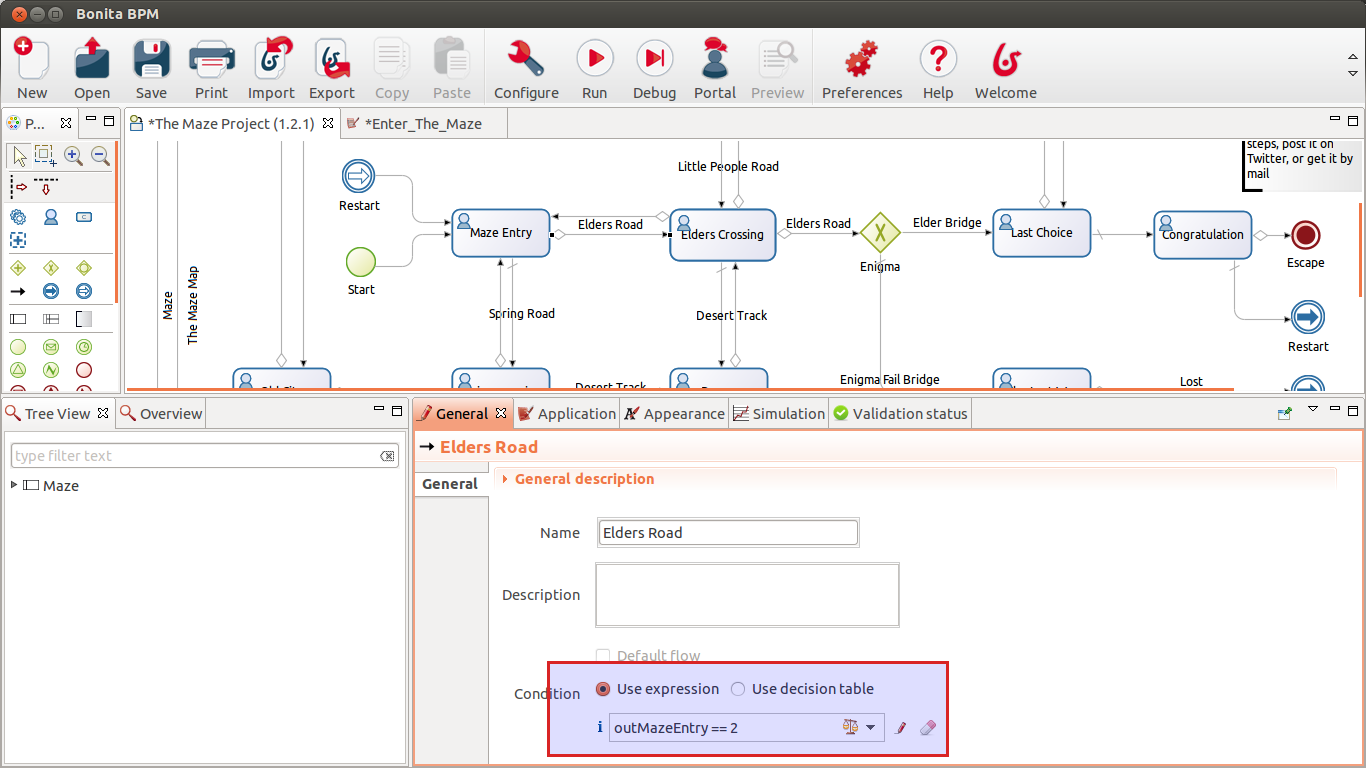
\includegraphics[width=14cm]{images/bonita.png}
\caption{
Screenshot von Bonita BPM
\newline
Quelle: {\protect\url{
http://i.imgur.com/ZY46h1R.png
}}\newline
Aufruf: 13.12.2017
}
}
\end{center}
\end{minipage}
\end{figure}

Bonita ist ebenfall, wie ARIS Express, eine Java-Anwendung wodurch sie auf allen
gängigen Betriebssystemen eingesetzt werden kann.

\subsection{Bizagi BPMN Modeler}
TODO
\subsection{ADONIS:Community}



 \\
Ldforem ips um do lor sit amet, consetetur sadipscing elitr, \label{Referenz}
sed diam  nonumy eirmod tempor invidunt ut labore et dolore magna aliquyam erat,
sed diam vddoluptsssua. At vero eos et accusam et justo duo dolores et ea rebum.
Stet clita kasd gubergren, no sea takimata sdner anctus est Lorem ipsum dolor sit amet. Lorem ipsum dolor sit amet, consetetur sadipscing elitr, sed diam nonumy eirmod tempor invidunt ut labore et dolore magna aliquyam erat, sed diam voluptua. At vero eos et accusam et justo duo dolores et ea rebum. Stet clita kasd gubergren, no sea takimata sanctus est Lorem ipsum dolor sit amet.
\footcite[Vgl.][Experto.de, Artikel über das und jenes]{praxishandbuch:bpmn2}
\subsubsection{Beispieltext}
Lorem ipsum dolor sit amet, co nsetetur sadipscing elitr, sed diam
nonumy eirmod tempor invidunt ut labore et dolore magna aliquyam erat, sed diam voluptua. At vero eos et accusam et justo duo dolores et ea rebum. Stet clita kasd gubergren, no sea takimata sanctus est Lorem ipsum dolor sit amet. Lorem ipsum dolor sit amet, consetetur sadipscing elitr, sed diam nonumy eirmod tempor invidunt ut labore et dolore magna aliquyam erat, sed diam voluptua. At vero eos et accusam et justo duo dolores et ea rebum. Stet clita kasd gubergren, no sea takimata sanctus est Lorem ipsum dolor sit amet.

%erzwinge Seitenumbruch
\clearpage

\subsection{Beispielbilder}
Lorem ipsum dolor sit amet, consetetur  sdf sadipscing elitr, sed diam nonumy eirmod tempor invidunt ut labore et dolore magna aliquyam erat, sed diam voluptua. At vero eos et accusam et justo duo dolores et ea rebum. Stet

\begin{center}
	
\includegraphics[width=5cm]{images/company_logo.png}
	\captionof{figure}{Beispielbild - Quelle: Internet}
\end{center}

Lorem ipsum dolor sit amet, consetetur sadipscing elitr, sed diam nonumy eirmod tempor invidunt ut labore et dolore magna aliquyam erat, sed diam voluptua. At vero eos et accusam et justo duo dolores et ea rebum. Stet
\begin{center}
	
\includegraphics[width=10cm]{images/institute_logo.png}
	\captionof{figure}{Beispielbild2 - Quelle: Internet}
\end{center}


\clearpage



\section{Die Kunst des Dönermachens}

Beispielzitat bei mehr als 2 Zeilen:
\begin{quote}
"`Döner macht schö2ner über mehr als 5 Zeilen\\
Macht Ali dir auch einen Döner \\
ohne Extra Soße \\
aber den Käse vergisst er trozdem\\
ENDE."' 
\footcite[Wörtlich übernommen von Ali]{praxishandbuch:bpmn2}
\end{quote}
Verweis innerhalb des Dokuments:\footcite[Vgl. \ref{Referenz} auf Seite
\pageref{Referenz} ]{testarticle}


\begin{figure}[H]
\begin{minipage}{\linewidth}
\begin{center}
\fbox{
\centering

\includegraphics[width=10cm]{images/company_logo.png}
\caption{
Schauerleute im Hamburger Hafen
\newline
Quelle: {\protect\url{
https://de.wikipedia.org/wiki/Hafenarbeiter#/media/File:Dockers\%27_work_difference.jpg
}}\newline
Aufruf: 13.10.2015
}
}
\end{center}
\end{minipage}
\end{figure}

\clearpage
\section{Anhang}

Lorem ipsum\ldots
